\documentclass[a4paper]{article}

\usepackage{hyperref}
\usepackage[utf8]{inputenc}
\usepackage[a4paper, margin=3.5cm]{geometry}
\usepackage{graphicx}
\usepackage{url}
\usepackage[spanish,es-tabla]{babel}
\usepackage{fancyhdr}
\usepackage{float}
\usepackage{booktabs}
\usepackage{multirow}
\usepackage[nolist]{acronym}
\usepackage[
    type={CC},
    modifier={by-nc-sa},
    version={3.0},
]{doclicense}

\renewcommand{\headrulewidth}{0.6pt}
\renewcommand{\footrulewidth}{0.6pt}

\pagestyle{fancy}
\setlength\headheight{50pt}
\lhead{
\includegraphics[height=1.5cm]{logos/upm_logo}}
\chead{Bases de Datos\\\vspace{.5em} Ejercicios procedimientos, funciones y triggers\\\vspace{-.1em}}
\rhead{
\includegraphics[height=1.5cm]{logos/etsisi_logo}}
\lfoot{\textbf{Tema 5:} Gestión de bases de datos}
\cfoot{}
\rfoot{\thepage}

\parskip 1.1ex % paragraph spacing

\begin{acronym}
    \acro{FIA}{Federación Internacional de Automovilismo}
\end{acronym}

\begin{document}
\section*{Carreras de Formula 1}

La \ac{FIA} está tratando de recopilar toda la información que han recogido en los últimos años durante las carreras de Fórmula 1. Con todos los datos que han conseguido recabar quieren realizar diversos estudios con el fin de mejorar el espectáculo. No obstante, antes de poder realizar ningún estudio se necesita crear una base de datos donde se pueda almacenar la información. 

Para ello, la compañía nos ha suministrado el Modelo Relacional que se muestra en la figura~\ref{fig:relacional}, con el fin de facilitar las pautas necesarias a tener en cuenta para poder crear la base de datos.

\begin{figure}[H]
  \centering
  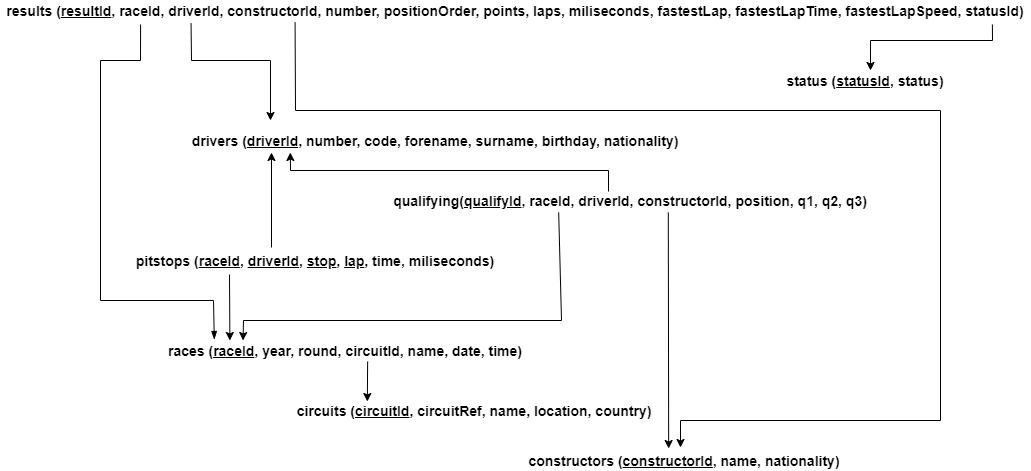
\includegraphics[width=\textwidth]{figs/modelo-relacional}
  \caption{Modelo relacional de la Fórmula 1.}
  \label{fig:relacional}
\end{figure}

Adicionalmente, se hace constar que este modelo tiene añadidas las siguientes restricciones:
\begin{itemize}
    \item Todos los identificadores se presentan de forma numérica.
    \item Los nombres, apellidos, nacionalidades y localizaciones no podrán exceder en ningún caso los 250 caracteres.
    \item Los campos que indican número de vuelta, puntos y velocidades tendrán que adaptarse como valores \texttt{INT}, \texttt{FLOAT} o \texttt{DOUBLE} según corresponda.
    \item Existen tres tipos adicionales de valores con formato temporal como son \textit{time} de tipo \texttt{TIME}, \textit{date} y \textit{birthday} de tipo \texttt{DATE} y \textit{year} de tipo \texttt{YEAR}.
\end{itemize}

Se desean implementar los siguientes procedimientos, funciones y triggers:

\begin{enumerate}
    \item Crea un procedimiento almacenado de nombre \texttt{getRacesInAYear}, que obtenga como salida los nombres de las carreras y el número total de constructores que han participado en la carrera, para un año concreto que se pasará como parámetro de entrada. En el procedimiento no se definirán parámetros de salida.  
    
    \item Se quiere testear los mensajes que se le envían a los pilotos por pantalla en plena carrera. Para ello se quiere crear un procedimiento de nombre \texttt{getOnRaceMessages}, que reciba un código de mensaje, e indique en un parámetro de salida el mensaje concreto teniendo en cuenta las siguientes condiciones:
    \begin{itemize}
        \item E01 = Error en la presión de las ruedas
        \item E02 = Pinchazo
        \item E03 = Temperatura alta en el motor
        \item E04 = Frenos sobre-calentados
        \item E05 = Error presión del aceite
        \item Cualquier otro valor = Error de comando
    \end{itemize}
            
    \item Crea un procedimiento que reciba una nacionalidad como parámetro de entrada y realice una consulta sobre la tabla \texttt{drivers} para obtener todos los pilotos de esa nacionalidad.
       
    \item Escribe una función que devuelva el número de puntos que se ha conseguido el campeón de ese año en cada mundial.
           
    \item Escribe una función que devuelva el valor medio de puntos por año que ha conseguido un determinado constructor que se recibirá como parámetro de entrada. El parámetro de entrada será el nombre del constructor.
            
    \item Escribe una función que dado el \texttt{driverId} de un piloto devuelva el número total de años en activo que ha estado compitiendo.
      
    \item Añade una nueva columna en la tabla \texttt{drivers} que se llame años en activo. A continuación escribir un procedimiento que calcule el número total de años que ha estado un piloto compitiendo y actualice la tabla. Este procedimiento hará uso de la función creada en un ejercicio anterior.
    
    \item A partir de este momento la FIA no va a permitir que haya equipos con más de 2 pilotos, por ello se debe desarrollar un trigger que impida que se puedan incorporar en un mismo equipo más de 2 pilotos a la base de datos. Para ello, se debe impedir toda operación que haga que un 3 o más pilotos pasen a formar parte del mismo equipo de constructores, ya sea mediante inserción o actualización de los datos. 
            
    \item Crea una tabla \texttt{crashes} con la siguiente estructura:
    \begin{table}[h]
    \centering
    \begin{tabular}{@{}lll@{}}
    \toprule
    \multicolumn{1}{c}{\textbf{driverId}} & \multicolumn{1}{c}{\textbf{crashId}} & \multicolumn{1}{c}{\textbf{Descripción}} \\ \midrule
                                          &                                      &                                          \\ \bottomrule
    \end{tabular}
    \end{table}

    Crea un trigger que cuando se inserte una fila en la tabla \texttt{results} con el parámetro \texttt{statusId} de valores 1, 2 o 3 rellene la tabla \texttt{crashes} con la información correspondiente.

    \item Crea un trigger para impedir que en un mismo año un piloto esté en dos equipos de constructores diferentes.
         
    \item Crea un procedimiento almacenado para obtener los pilotos y los circuitos que ganaron carreras de un año concreto (como argumento) con un constructor del mismo país que el piloto.

    \item Escribe un procedimiento que realice la selección de aquellos pilotos que en el año que se le pase como parámetro de entrada, obtuvieron un primer, un segundo y un tercer puesto.
        
    \item Codifique una función almacenada llamada \texttt{diffPoints} que reciba los identificadores de dos pilotos como parámetros (\texttt{driver1} y \texttt{driver2}) y devuelva la diferencia de puntos totales conseguidos por \texttt{driver1} con respecto de \texttt{driver2}. Tenga en cuenta que el valor será positivo si \texttt{driver1} ha conseguido más puntos que \texttt{driver2}  y negativo en caso contrario.
    
    \item Cree una nueva tabla \textit{sponsors} en la base de datos que almacene como atributos, su identificador propio, su nombre, tipo, el identificador de la carrera que patrocina y el dinero que aporta anualmente. Luego, diseñe un trigger para la nueva tabla \textit{sponsors}. Cada carrera puede contar con varios patrocinadores, los cuales se dividen en dos tipos, oficiales (deben aportan una cantidad igual o superior a 5M de euros anuales) y cooficiales (cantidades inferiores). Diseñe un trigger que clasifique al sponsor y rellene el atributo \textit{type} de su correspondiente tabla. Ten en cuenta que un sponsor puede cambiar de año en año la cuantía que aporta.

    \item Procedimiento almacenado de nombre \texttt{getsConstructoresYPilotos}, que tomando como entrada un año concreto, obtenga como salida los nombres de todos los pilotos que participaron en el mundial ese año y el equipo de constructores con el cual compitieron. Adicionalmente, también se quiere obtener el total de puntos que obtuvo cada piloto en el mundial.

    \item Codifique un procedimiento llamado \texttt{getNumberOfVictories} que disponga de un parámetro de entrada \texttt{type}. Si \texttt{type = 'nationality'}, el procedimiento listará el número de victorias que han obtenido cada una de las nacionalidades de la tabla \texttt{drivers}. Por contra, si \texttt{type} toma cualquier otro valor, el procedimiento listará el número de victorias que han obtenidos cada uno de los constructores (\texttt{constructors.name}) existentes en la base de datos. Los resultados deberá estar ordenados de mayor a menor número de victorias.
\end{enumerate}

\vspace{2em}
\hrule
\doclicenseThis

\end{document}
